\chapter{データベースを使わない世界}

データベースと聞いて何を思い浮かべるだろうか.
大抵の人は,データベースといえば「大きなデータの集まり」といったイメージを持つのではないだろうか.
このイメージはあながち間違いではない.

さて,本講義のようにわざわざ科目を立ててまで,データベースについて学ぶことはあるのだろうか?
結論としては,大規模データに携わるITエンジニアやデータ分析者を目指す人であれば,「大いにあり」である.
1960年代から今日に至るまで,データベース技術は盛んに研究開発が行われてきた.
大きなデータの集まりを扱うには,対処しなければならない問題が思った以上に数多く存在するのである.

本講義では10数回にわたってデータベース技術について解説するが,この第1講ではデータベースのことはいったん横に置いておいておく.
今回は(割と)大きなデータを扱うときに遭遇する問題について考えてみよう.


% ---------------------------------------
\section{ケース1: 販売履歴の記録をはじめる}
% ---------------------------------------
以下は,山畑さんという架空の人物のお話である.

\begin{framed}
山畑さんは家族で小さな小売店を営んでいる.
個人経営ながら山畑さんのお店は繁盛している.
とはいえ,街には大手チェーン小売店が進出してきており,このまま順調に経営を続けられるか,不安が募っている.
何か手を打たなければならない.

2020年の4月,山畑さんは念願のショッピングサイトを立ち上げた.
言うまでもない.
ショッピングサイトを立ち上げたのは,オンラインの場にも顧客獲得の機会を求めるためだ.
サイトは順調に立ち上がり,注文もポツポツ入ってきている.

ところで,最近「データサイエンス」なるものが世間の注目を集めているらしい.
データを活かせばビジネスチャンスが広がるとのことだ.
山畑さんは,Excelシートに記録を取り始めた販売履歴を分析してみようと思い立った.

山畑さんが使っているExcelシートには,「いつ,誰が,何を,いくらで購入したか」の情報が記録されている.
ショッピングサイトは立ち上がったばかりであり,Excelシートには200行しかデータが入っていない.
しかし,今後データが貯まっていけば,売り上げを増やすための課題が見えるかもしれない.
いずれがっつりとデータ分析をやるためにも,山畑さんは手持ちのデータを用いて分析の練習に取り組むことにした.
\end{framed}


\subsubsection{Q1. データの確認}
こちらのURL(\url{https://dbnote.hontolab.org/data/purchase\_small.xlsx})から,上のケース1で山畑さんがデータ分析の練習に使おうとしているExcelファイル(\graybox{purchase\_small.xlsx})をダウンロードし,中身を確認しなさい.

なお,Excelシートの各列の意味は以下の通り:
\begin{itemize}
\item purchased\_at: 購買(販売)日時
\item customer: 商品を購入した人物の氏名
\item gender: 商品を購入した人物の性別
\item product: 購入された商品名
\item sale: 販売価格
\end{itemize}


\subsubsection{Q2. あの人は何回買い物をしている?}
「岡田 真綾」という人物が何回買い物をしていたかを数えなさい.


\subsubsection{Q3. 商品Xを購入しているのは誰?}
Excelのオートフィルタ機能を使って,「ビタミン補助剤」を購入している人をリストアップしなさい.


\subsubsection{Q4. 総売上金額}
Excel関数の\graybox{\texttt{SUM}}を用いて,現時点での総売上金額を計算しなさい.


\subsubsection{Q5. 最も売れた商品は?}
Excelのピボットテーブル機能を使って,集計期間中に
\begin{itemize}
\item 最も購買回数が多かった商品
\item 最も売上金額の合計が大きかった商品
\end{itemize}
をそれぞれ求めなさい.



% ---------------------------------------
\section{ケース2: サイトの認知度向上につき,得られるデータも膨大に!?}
% ---------------------------------------
現時点では手持ちのデータは少ないものの,販売履歴データの分析に将来性を感じた山畑さん.
販売履歴データを有効活用できるよう,ショッピングサイト運営により力を入れる決意を固めたのであった.

以下は,山畑さんのその後の話(架空の話)である.

\begin{framed}
ショッピングサイト立ち上げ以降,順調に利用者数も増えていった.
やはりメディアに取り上げられたのが大きかったのだろう.
あのタイミングでサイトの認知度が一気に高まり,サイトの利用者数や利用頻度も加速度的に増えていった.
それに伴い,サイト運営に関わるスタッフも増員した.

販売履歴の管理は,当初は山畑さんが一人で担当していたが,さすがに一人では対応しきれなくなった.
そこで,ある時点から数名体制で販売履歴の記録を行うことになった.
これまで販売履歴の管理に使ってきたExcelシートをクラウドストレージに置き,記録担当スタッフのPC間で同期を取る仕組みを導入.
同じExcelファイルの上で,スタッフ全員で販売履歴を記録できるようにしたのである.

2年後.サイト事業は軌道に乗った.
十分な量の販売履歴データが蓄積されたと判断した山畑さんは,いよいよ大規模な販売履歴データの分析に取りかかることを決意した.
立ち上げ当初は200〜300行しかなかったExcelシートであったが,シートを開きその行数を数えてみると…
なんとその数90万行以上!
データの量に小躍りした山畑さんは,Excelシートの扱いに詳しいスタッフと共に,意気揚々とデータ分析に取りかかったのであった.
\end{framed}


\subsubsection{Q6. データの再確認}
こちらのURL(\url{https://dbnote.hontolab.org/data/purchase\_large.xlsx})から,上のケース2で山畑さんが分析しようとしているExcelファイル\graybox{purchase\_large.xlsx}をダウンロードしなさい.
またダウンロードしたファイルを用いて下記課題(演習1と同じ)に取り組み,データ分析上の課題(困ったこと)を議論しなさい.
以下,課題1の内容を再掲する.
\begin{itemize}
    \item 「岡田 真綾」という人物が何回買い物をしていたかを数えよ
    \item 「ビタミン補助剤」を購入している人をリストアップせよ
    \item 総売上金額を計算せよ
    \item 集計期間中に「最も購買回数が多かった商品」「最も売上金額の合計が大きかった商品」を求めよ
    \end{itemize}
もし,\graybox{purchase\_large.xlsx}ファイルがうまく開けない場合は,こちらのURL(\url{https://dbnote.hontolab.org/data/purchase\_medium.xlsx})からダウンロードできる\graybox{purchase\_medium.xlsx}を用いなさい.
なお,ダウンロードできるExcelシートの構造はケース1で用いた\graybox{purchase\_small.xlsx}と同じである.


% ---------------------------------------
\section{表計算ソフトでデータ管理を行ったときに起きる悲劇}
% ---------------------------------------
ケース1および2で用いたExcelファイルは,販売履歴データの集まりであった.
一般的な認識からすると,このようなデータの集まりは「データベース」ということになるだろう.

ところで,上記演習,とりわけケース2に取り組んでみてイライラしなかっただろうか?
数万件,数十万件ある表データをExcelで扱おうとすると,さまざまな不都合が生じる(図\ref{fig:excel-disaster}).
これは,本来Excelは個人用の表計算アプリケーションであって,大規模データの管理や処理を前提として設計されていないためである.

\begin{figure}[tb]
    \centering
    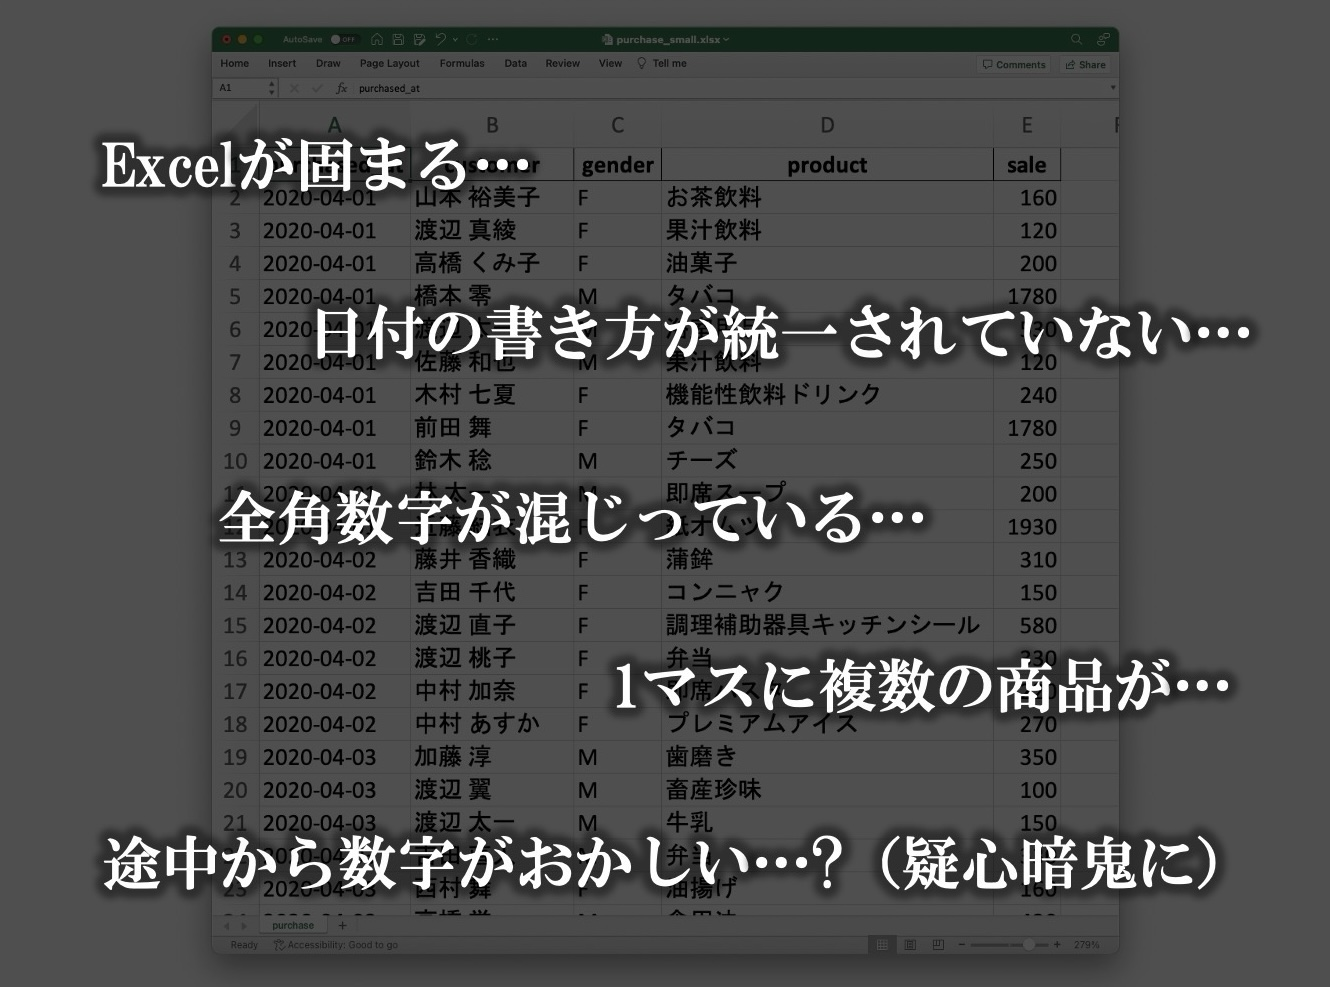
\includegraphics[width=0.8\textwidth]{figure/excel-disaster.jpg}
    \caption{大きな表データを複数人でExcelで扱うときの悲劇.}
    \label{fig:excel-disaster}
\end{figure}

では,大規模なデータを管理・処理するためにはどうすればよいだろうか?
そのための技術こそが「データベース」である.
以降,本書では\strong{大規模データを効率よく管理・処理するための「データベース」技術} について学習する.

